\newcommand{\DoNotLoadEpstopdf}{}
\documentclass[11pt,letterpaper]{article}
\usepackage[utf8]{inputenc}
\usepackage[T1]{fontenc}
\usepackage{lmodern}
\usepackage{geometry}
\usepackage{graphicx}
\usepackage{booktabs}
\usepackage{array}
\usepackage{longtable}
\usepackage{float}
\usepackage{xcolor}
\usepackage{hyperref}
\usepackage{amsmath}

\geometry{top=2.1cm,bottom=2.2cm,left=2.35cm,right=2.35cm}
\definecolor{navy}{HTML}{102A43}
\definecolor{blue}{HTML}{2563EB}
\definecolor{teal}{HTML}{0F9D91}
\definecolor{soft}{HTML}{F1F5F9}
\definecolor{red}{HTML}{DC2626}
\hypersetup{
  colorlinks=true,
  linkcolor=navy,
  urlcolor=blue,
  citecolor=teal,
  pdftitle={Laboratorio 5 - Mineria de Textos y Analisis de Sentimientos},
  pdfauthor={Grupo 1, Data Science, Seccion 10}
}
\setlength{\parindent}{0pt}
\setlength{\parskip}{0.55em}
\setlength{\emergencystretch}{3em}
\renewcommand{\arraystretch}{1.18}
\newcommand{\metric}[2]{\textcolor{navy}{\textbf{#1}} & #2 \\}
\newcommand{\repo}{\href{https://github.com/DanielBarillasM/Laboratorio-5.-Mineria-de-Textos-y-Analisis-de-Sentimientos_Grupo-1_DS_Sec-10}{Repositorio oficial del Laboratorio 5}}

\begin{document}

\begin{titlepage}
\pagecolor{navy}
\color{white}
\centering
\vspace*{1.8cm}
{\small UNIVERSIDAD DEL VALLE DE GUATEMALA\par}
\vspace{0.35cm}
{\small DATA SCIENCE · SECCIÓN 10 · GRUPO 1\par}
\vfill
{\Huge\bfseries Laboratorio 5\par}
\vspace{0.4cm}
{\LARGE Minería de Textos y\par Análisis de Sentimientos\par}
\vspace{0.8cm}
{\large Clasificación reproducible de tweets sobre desastres reales\par}
\vfill
\begin{tabular}{rl}
\textbf{Jorge Gabriel Palacios Sales} & 231385\\
\textbf{Pablo Daniel Barillas Moreno} & 22193\\
\textbf{Roberto Emiliano Otoniel} & 23968\\
\end{tabular}
\vfill
{\large Entrega final · 2026\par}
\vspace{0.5cm}
{\small \repo\par}
\end{titlepage}
\nopagecolor
\color{black}

\tableofcontents
\newpage

\section{Resumen ejecutivo}

Este trabajo desarrolla un flujo reproducible de procesamiento de lenguaje natural para identificar si un tweet describe un desastre real. Se analizaron las 7,613 observaciones etiquetadas de la competencia \emph{Natural Language Processing with Disaster Tweets} de Kaggle \cite{kaggle}. El proceso incluye validación de datos, limpieza auditable, frecuencias y n-gramas por clase, análisis exploratorio, comparación de clasificadores, inferencia sobre texto crudo, análisis de sentimiento con VADER, contraste estadístico, ingeniería de una variable de negatividad y análisis de errores.

La regresión logística con TF--IDF de unigramas y bigramas fue seleccionada como modelo final. En una partición estratificada 80/20 alcanzó exactitud de 0.813, F1 de 0.781 para la clase desastre y ROC--AUC de 0.867. Los tweets de desastre tuvieron negatividad media de 0.337, frente a 0.213 en los demás; la diferencia fue estadísticamente significativa, aunque de magnitud pequeña. Agregar la negatividad al clasificador redujo el F1 a 0.764, por lo que esta variable no se incluyó en el modelo definitivo.

\section{Objetivos}

\subsection{Objetivo general}

Aplicar técnicas de minería de textos, aprendizaje automático y análisis de sentimiento para describir y clasificar tweets relacionados con desastres reales.

\subsection{Objetivos específicos}

\begin{enumerate}
  \item Describir la estructura, calidad y distribución del conjunto de entrenamiento.
  \item Diseñar una limpieza de texto explicable y reproducible.
  \item Comparar vocabulario, unigramas, bigramas y trigramas entre clases.
  \item Evaluar varios clasificadores bajo una partición común.
  \item Implementar una función que reciba un tweet crudo y devuelva su clasificación.
  \item Etiquetar el sentimiento como positivo, negativo o neutral, conservando emoticonos y señales de superficie.
  \item comparar los diez tweets más positivos y negativos y determinar si los desastres se expresan con mayor negatividad.
  \item Incorporar una variable cuantitativa de negatividad, reentrenar el modelo y medir su aporte incremental.
\end{enumerate}

\section{Datos y protocolo experimental}

\subsection{Fuente y estructura}

El archivo principal es \texttt{data/raw/train.csv}, proveniente de Kaggle \cite{kaggle}. Su integridad se controla mediante SHA--256: \texttt{61111c6dc31eaffa34d1e1fa62e2395325c9bc3b38bba1941a5f1ed9b3fa60df}. Contiene las variables \texttt{id}, \texttt{keyword}, \texttt{location}, \texttt{text} y \texttt{target}. La variable objetivo vale uno cuando el tweet describe un desastre real y cero en caso contrario.

De las 7,613 observaciones, 4,342 (57.06\%) pertenecen a la clase sin desastre y 3,271 (42.94\%) a la clase desastre. Hay 61 valores ausentes en \texttt{keyword} y 2,533 en \texttt{location}; no hay valores faltantes en texto u objetivo. El archivo \texttt{test.csv} se conserva por trazabilidad, pero no se utiliza para evaluación porque no posee \texttt{target}.

\begin{figure}[H]
\centering
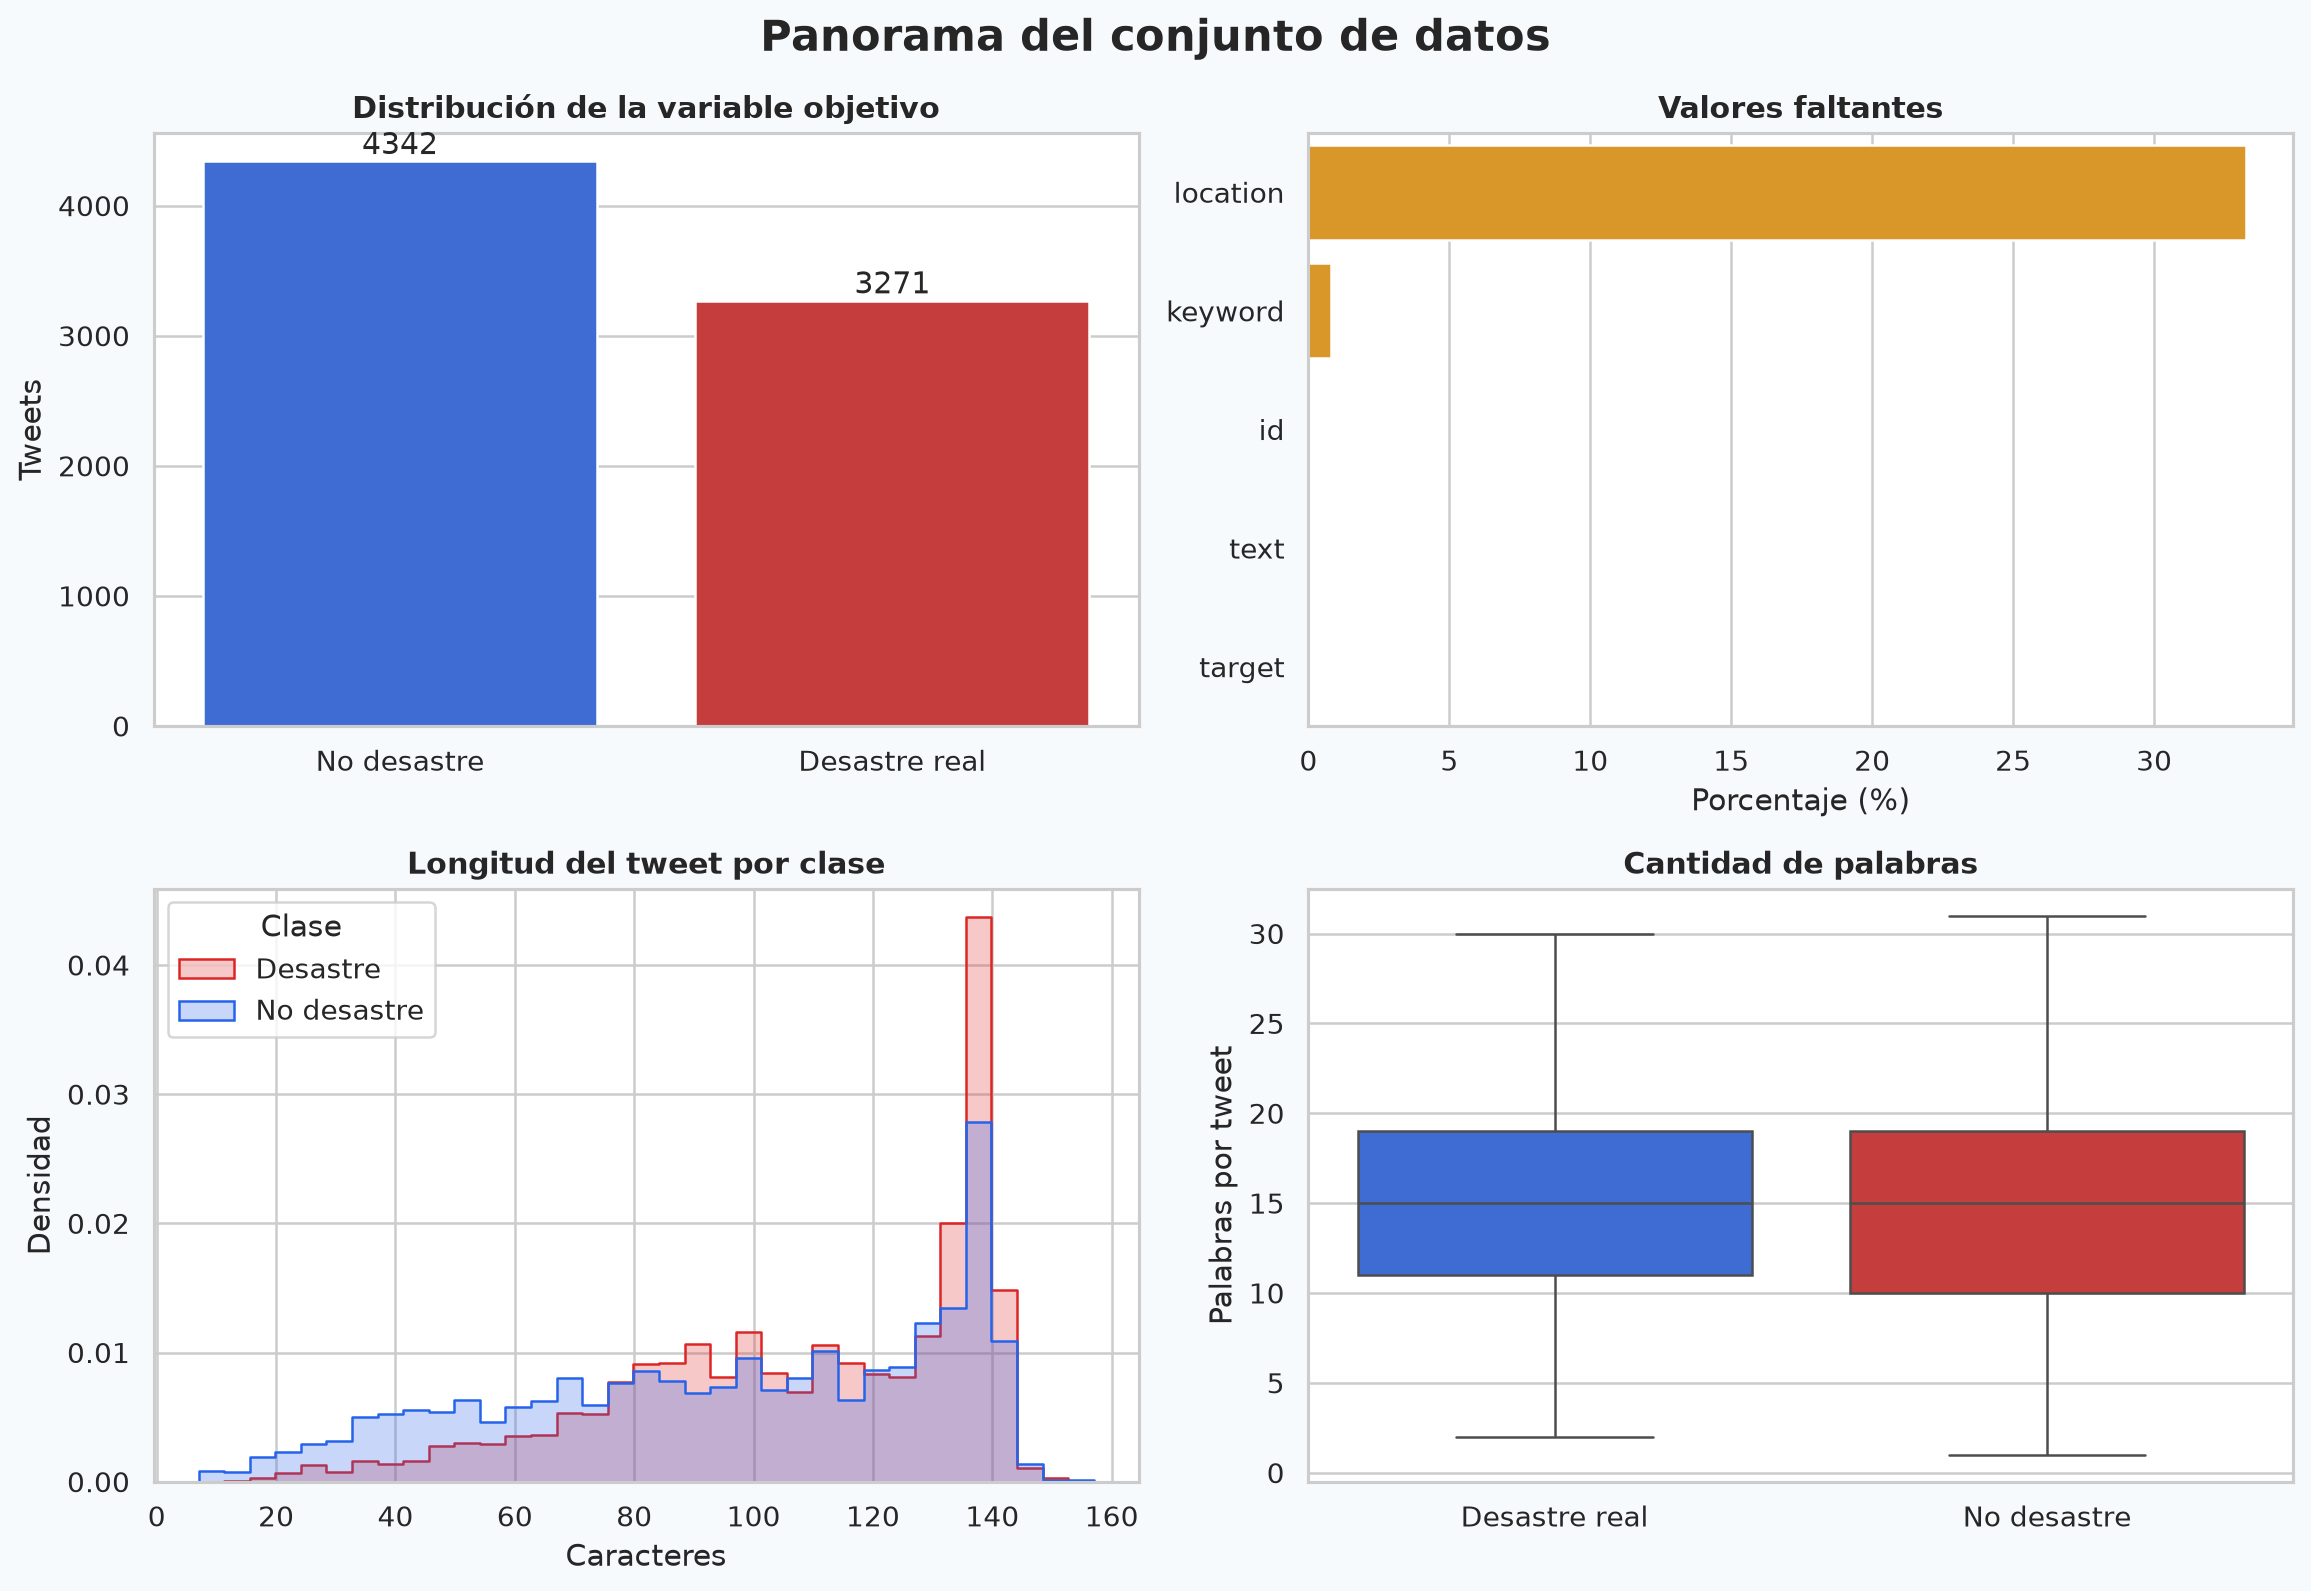
\includegraphics[width=0.97\textwidth]{../outputs/figures/eda_panorama.png}
\caption{Panorama del conjunto: distribución de clases, longitud del texto y variables faltantes.}
\label{fig:eda}
\end{figure}

\subsection{Partición y métricas}

Se realizó una separación estratificada con 80\% para entrenamiento (6,090 tweets) y 20\% para validación (1,523 tweets), usando semilla 42. Todos los modelos reciben exactamente las mismas observaciones. Debido al desbalance moderado se reportan exactitud, precisión, recall, F1 de la clase desastre, F1 macro y ROC--AUC. También se conservan las matrices de confusión.

\section{Limpieza y representación}

Para el clasificador se aplicaron los siguientes pasos:

\begin{enumerate}
  \item conversión a minúsculas y normalización Unicode;
  \item sustitución de URL y menciones por marcadores semánticos;
  \item separación del símbolo de los hashtags para conservar su palabra;
  \item eliminación de caracteres no informativos y reducción de espacios;
  \item eliminación controlada de palabras vacías;
  \item vectorización TF--IDF con unigramas y bigramas.
\end{enumerate}

La implementación de la limpieza utiliza los módulos estándar \texttt{re}, \texttt{html} y \texttt{string}, junto con \texttt{ENGLISH\_STOP\_WORDS} de \texttt{sklearn.feature\_extraction.text}. Para sentimiento se usa una normalización más ligera. No se eliminan negaciones, mayúsculas, signos de exclamación, emojis ni emoticonos, porque VADER utiliza esas señales para ajustar la intensidad \cite{vader}. El repositorio incluye \texttt{auditoria\_limpieza.csv}, ejemplos antes/después y una auditoría de la lista Glasgow de palabras vacías. Esta última revela que términos temáticos como \emph{fire} podrían ser eliminados; el efecto se declara como limitación y se mantiene constante en todas las comparaciones.

\section{Frecuencias y n-gramas}

Se calcularon conteos y probabilidades condicionales para unigramas, bigramas y trigramas dentro de cada clase. Los términos aislados permiten reconocer temas dominantes, mientras que los n-gramas recuperan contexto: una palabra como \emph{disaster} puede aparecer en una emergencia o como metáfora. Las expresiones asociadas con evacuación, incendios, advertencias y daños se concentran en la clase positiva; en la negativa aparecen usos sociales, promocionales y figurados.

\begin{figure}[H]
\centering
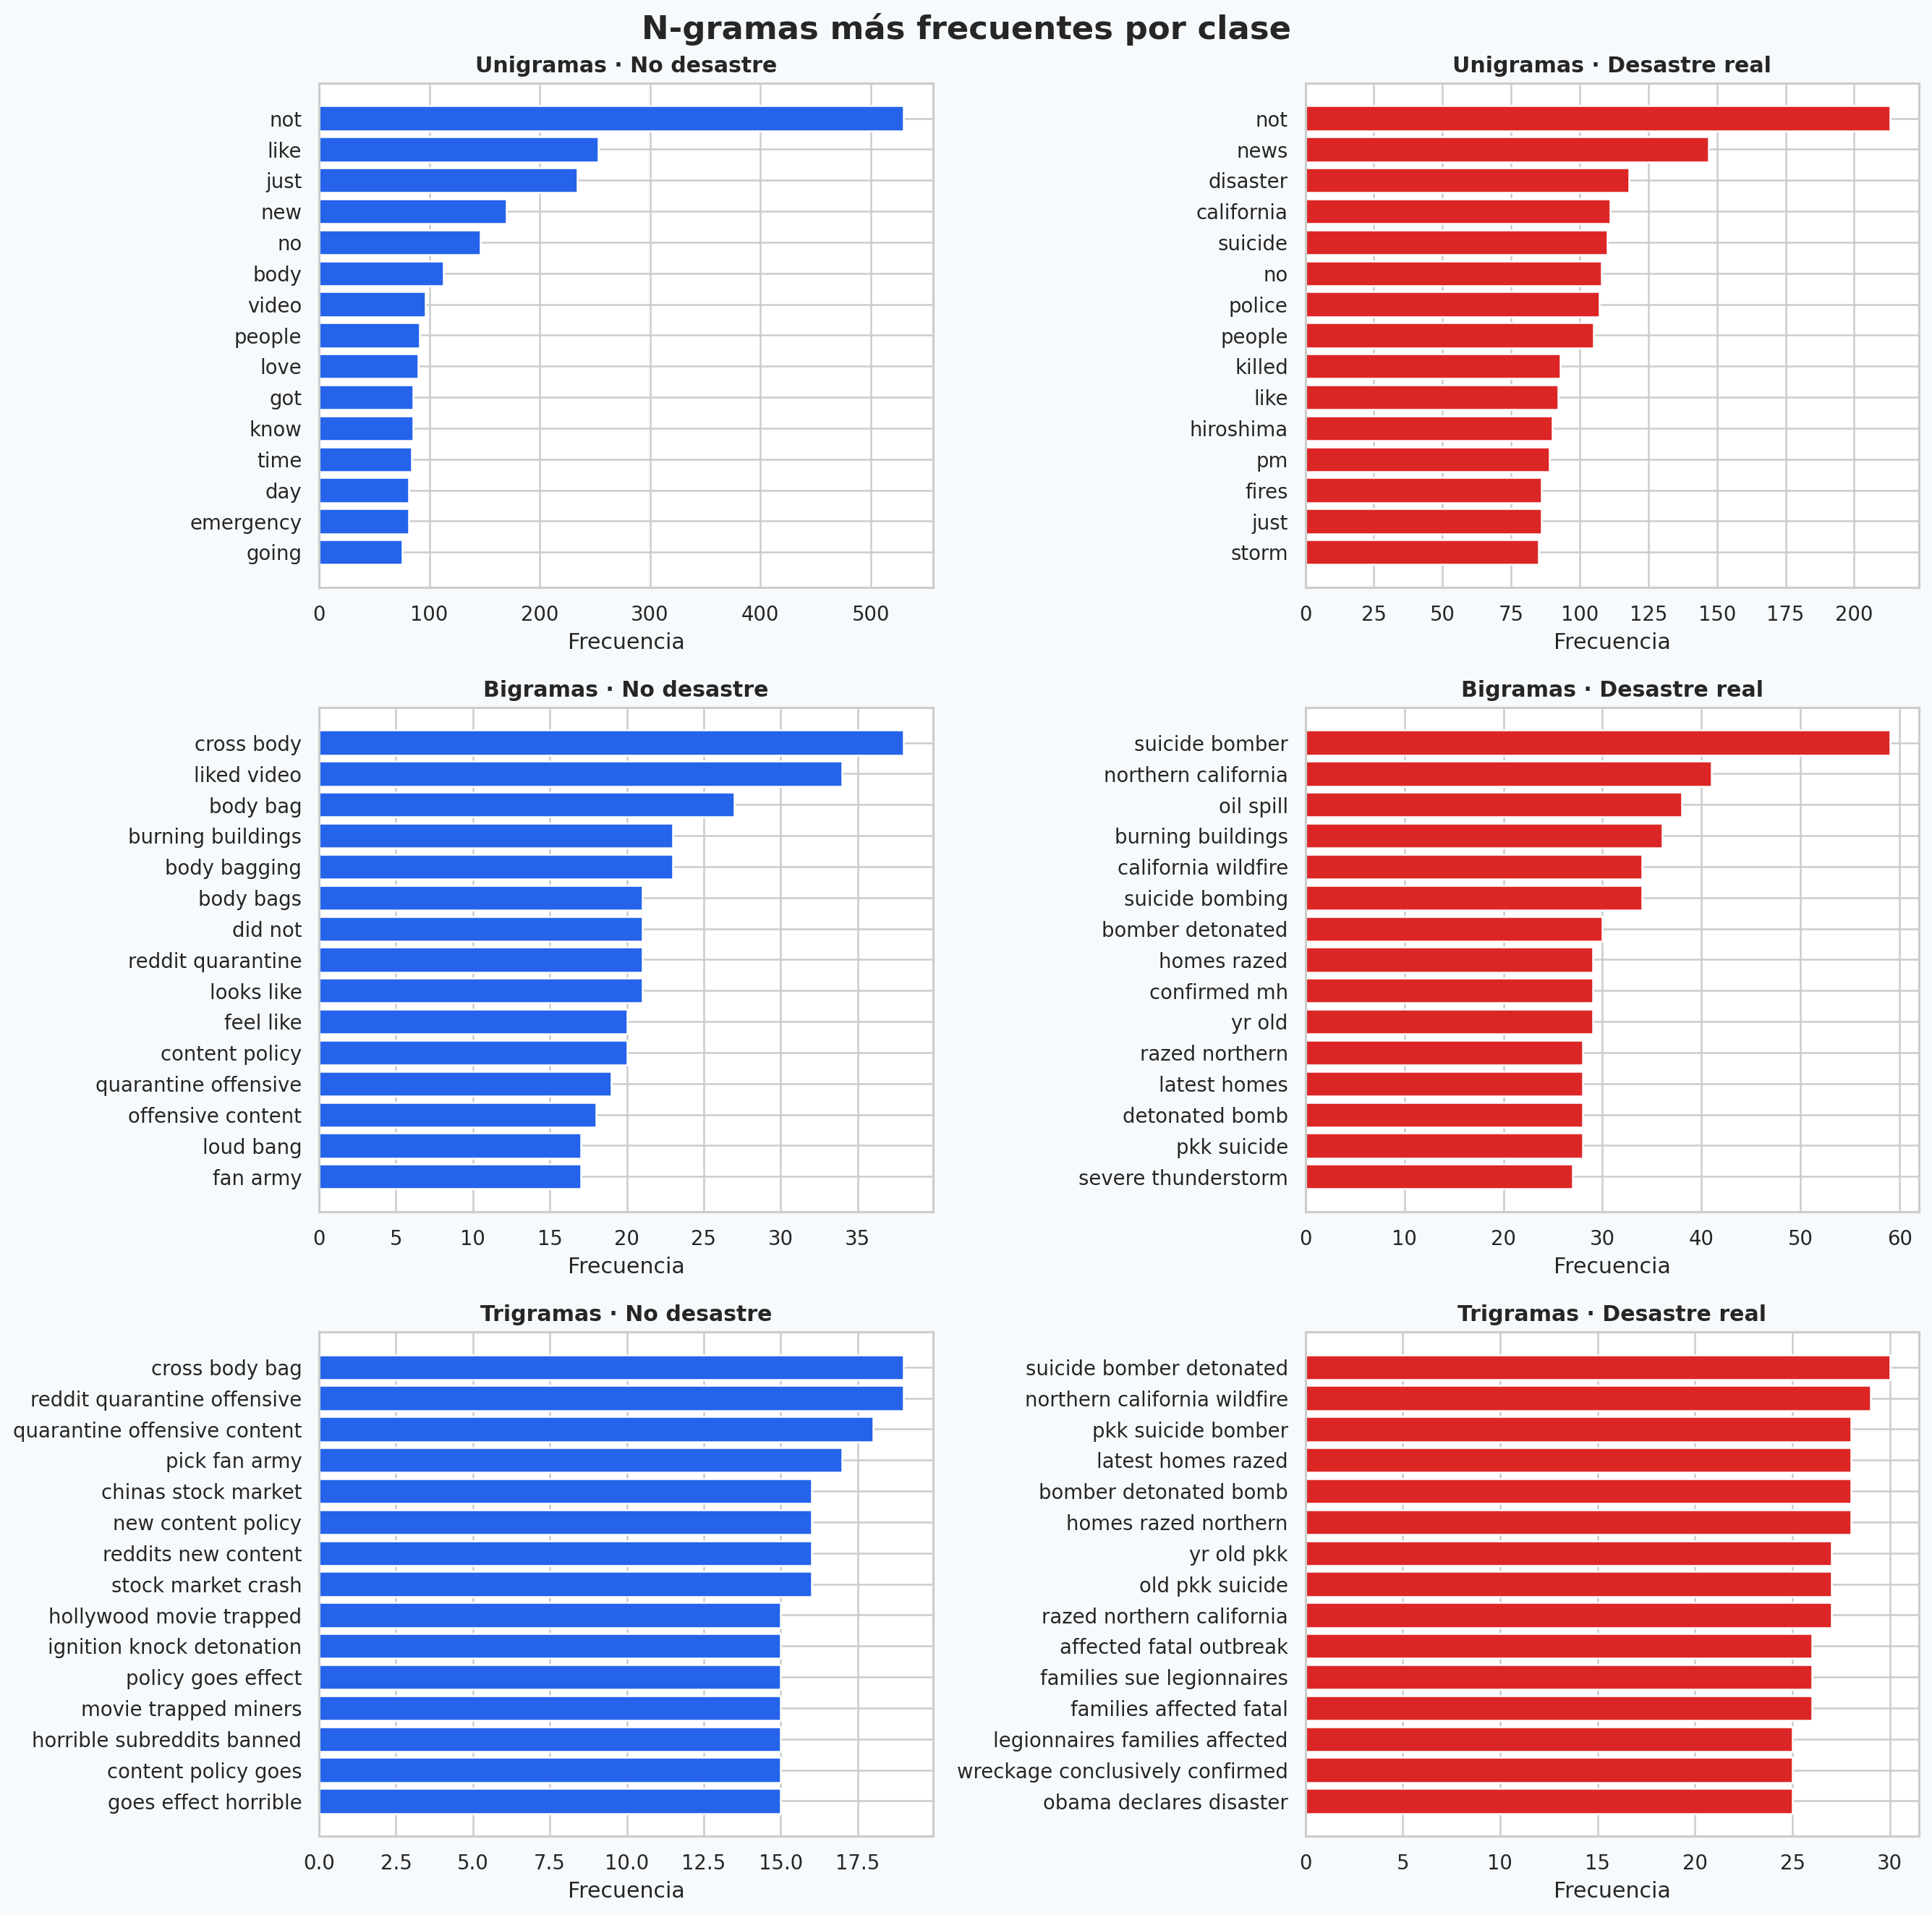
\includegraphics[width=0.98\textwidth]{../outputs/figures/ngramas_por_clase.png}
\caption{N-gramas principales por clase. Las probabilidades se calculan dentro de cada grupo.}
\label{fig:ngrams}
\end{figure}

Las nubes de palabras de la Figura \ref{fig:clouds} sirven como resumen visual, no como evidencia inferencial. La comparación cuantitativa se conserva en los CSV de \texttt{outputs/tables}.

\begin{figure}[H]
\centering
\begin{minipage}{0.49\textwidth}\centering
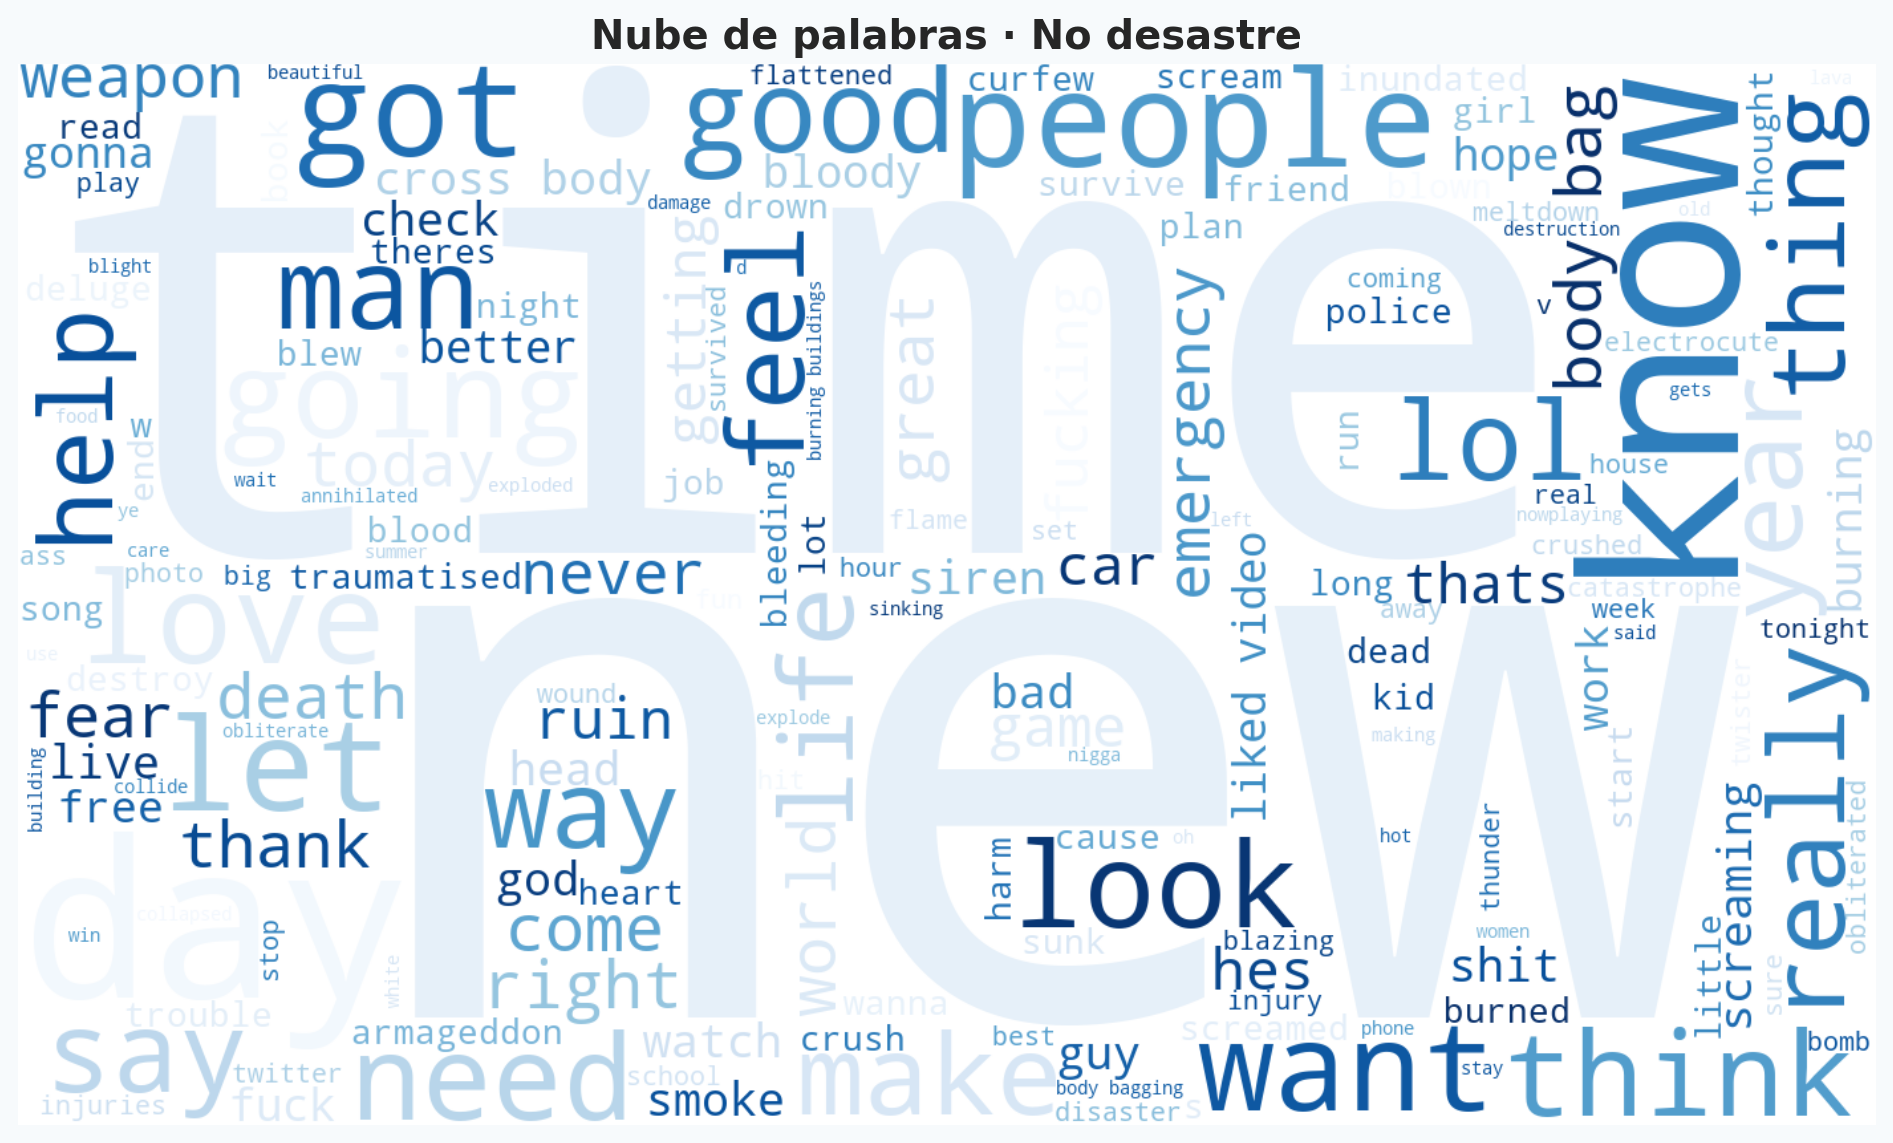
\includegraphics[width=\textwidth]{../outputs/figures/nube_palabras_target_0.png}
\small (a) No desastre
\end{minipage}
\begin{minipage}{0.49\textwidth}\centering
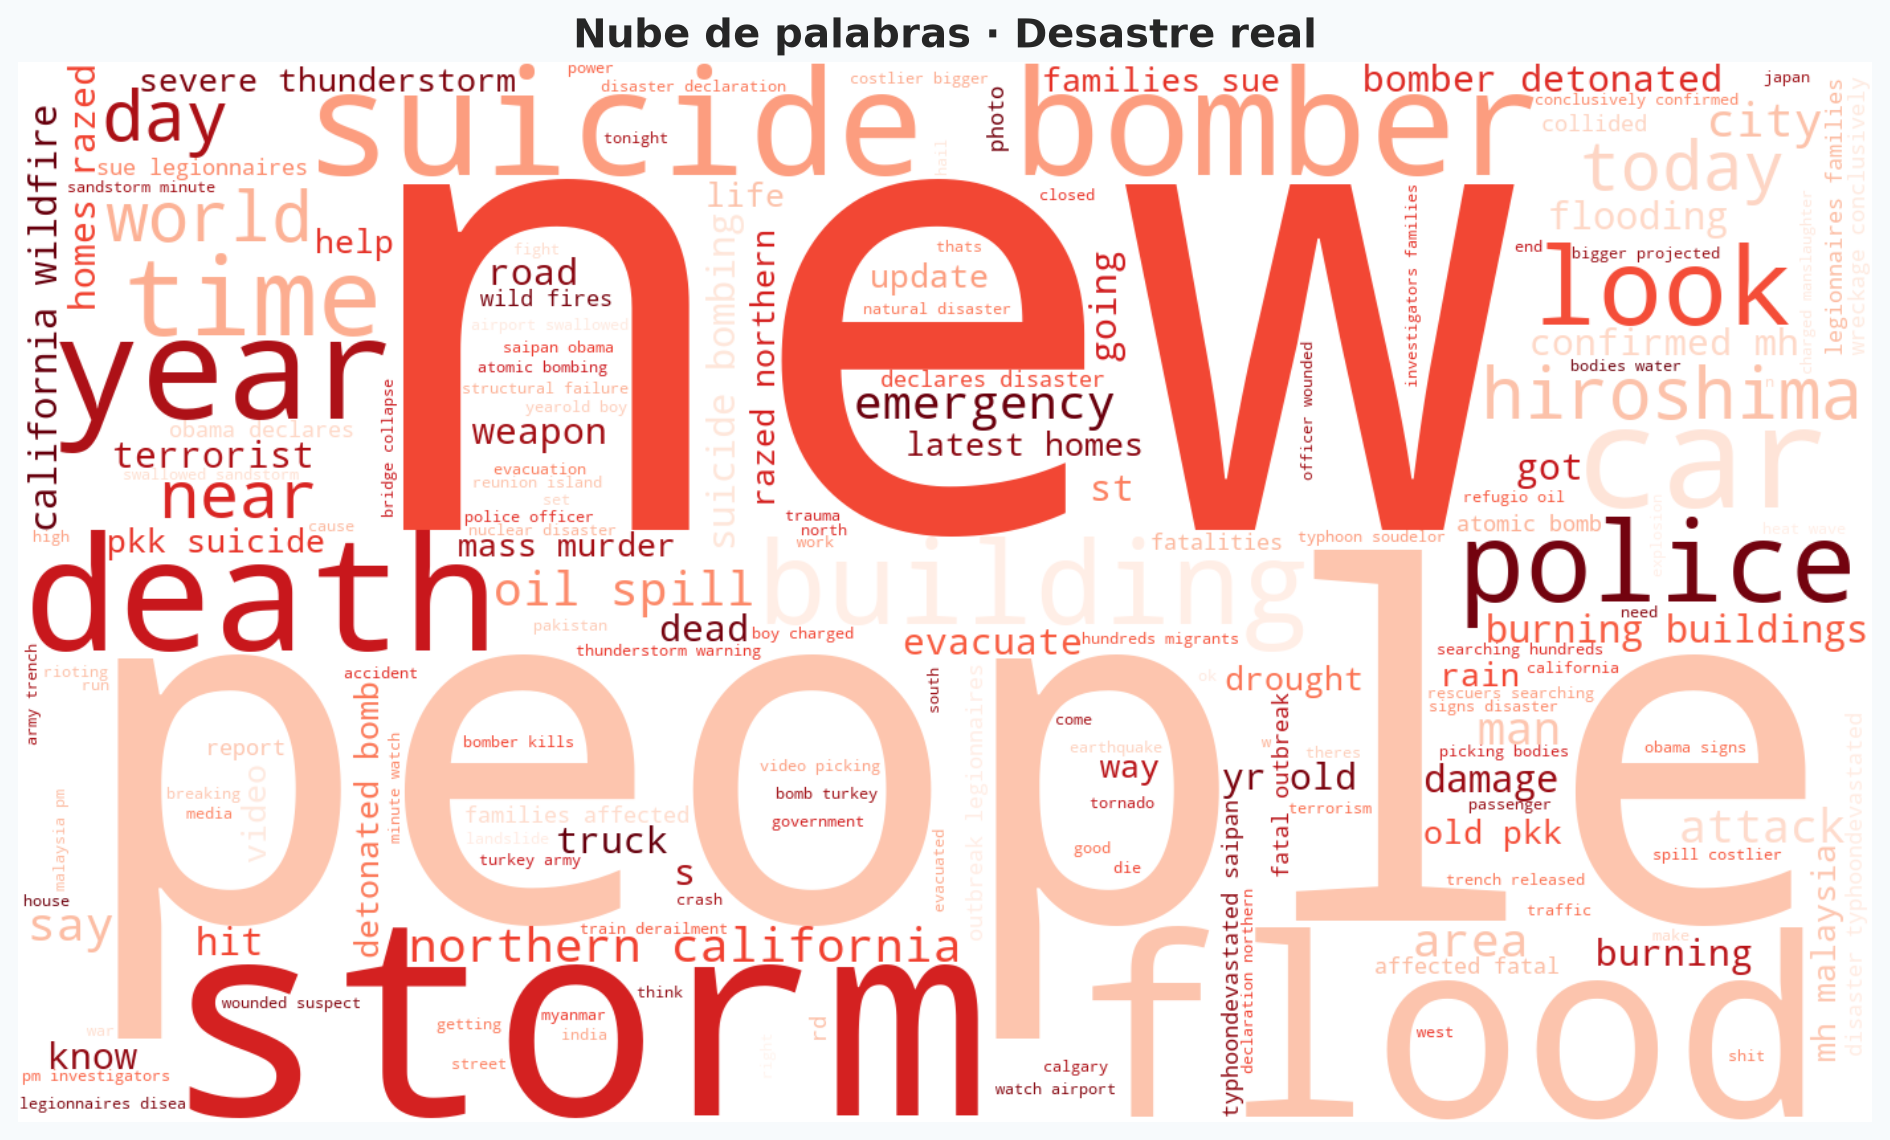
\includegraphics[width=\textwidth]{../outputs/figures/nube_palabras_target_1.png}
\small (b) Desastre real
\end{minipage}
\caption{Nubes de palabras por clase después de la normalización.}
\label{fig:clouds}
\end{figure}

\section{Modelado supervisado}

\subsection{Modelos comparados}

Se evaluaron cuatro alternativas: baseline de clase mayoritaria, Naive Bayes complementario, regresión logística y SVM lineal calibrado. Los tres clasificadores textuales se implementaron con las herramientas de scikit-learn \cite{sklearn}; la ponderación TF--IDF sigue el principio de dar mayor importancia a términos informativos y menos peso a palabras muy frecuentes \cite{tfidf}.

Todos los candidatos utilizaron la misma partición estratificada 80/20 con semilla 42. La representación TF--IDF empleó unigramas y bigramas (\texttt{ngram\_range=(1,2)}), \texttt{min\_df=2}, \texttt{max\_df=0.98}, ponderación sublineal y un máximo de 35,000 características. El Naive Bayes complementario usó \texttt{alpha=0.5}; la regresión logística, \texttt{C=2.0}, pesos de clase balanceados y \texttt{max\_iter=2000}; y el SVM lineal calibrado, \texttt{C=0.75}, pesos balanceados y calibración sigmoide en tres particiones. Estos parámetros se conservaron durante la comparación para garantizar trazabilidad y reproducibilidad.

\begin{table}[H]
\centering
\caption{Métricas en la partición de validación.}
\label{tab:modelos}
\small
\begin{tabular}{lrrrrrr}
\toprule
Modelo & Exactitud & Precisión & Recall & F1 & F1 macro & ROC--AUC\\
\midrule
Baseline mayoritario & 0.5706 & 0.0000 & 0.0000 & 0.0000 & 0.3633 & 0.5000\\
Naive Bayes & 0.8070 & 0.8000 & 0.7339 & 0.7656 & 0.8007 & 0.8636\\
Regresión logística & \textbf{0.8129} & 0.7852 & \textbf{0.7768} & \textbf{0.7809} & \textbf{0.8088} & \textbf{0.8666}\\
SVM calibrado & 0.8096 & \textbf{0.8074} & 0.7309 & 0.7673 & 0.8031 & 0.8613\\
\bottomrule
\end{tabular}
\end{table}

La regresión logística fue seleccionada por su mayor F1 y su equilibrio entre falsos positivos y negativos. El baseline demuestra que la exactitud aislada es insuficiente: alcanza 57.06\% sin identificar un solo desastre.

\begin{figure}[H]
\centering
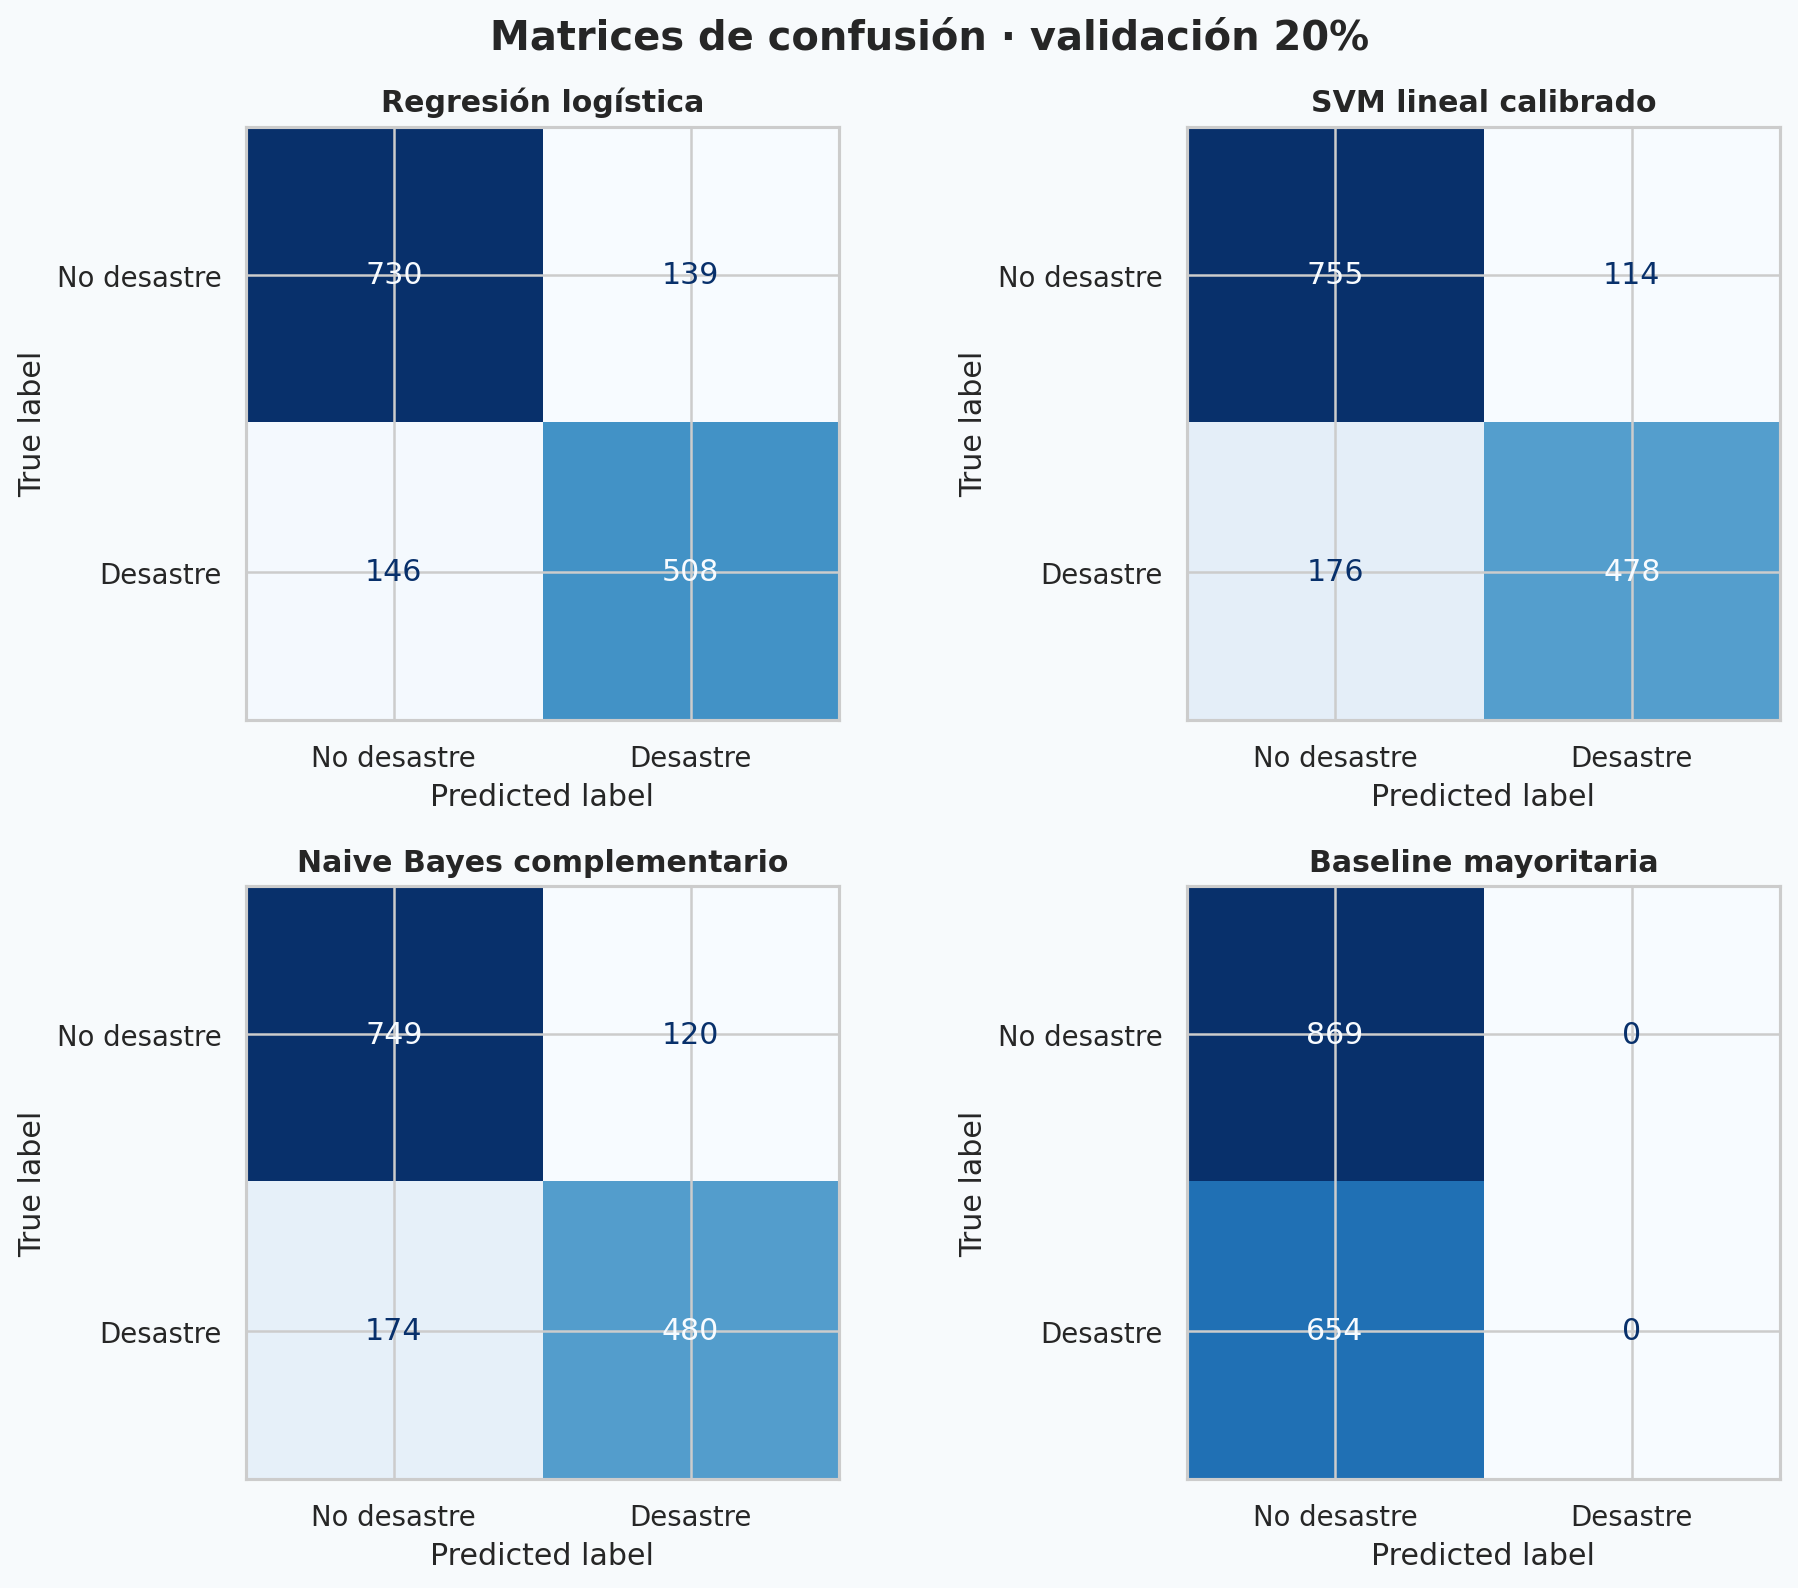
\includegraphics[width=0.98\textwidth]{../outputs/figures/modelos_matrices_confusion.png}
\caption{Matrices de confusión de los modelos comparados.}
\label{fig:confusion}
\end{figure}

\subsection{Función de clasificación}

La función \texttt{classify\_raw\_tweet} recibe un texto sin preprocesar. Internamente genera la versión limpia, calcula sentimiento y negatividad, ejecuta el pipeline persistido y devuelve clase, etiqueta, probabilidad de desastre y variables de sentimiento. El script \texttt{scripts/predict\_tweet.py} expone esta funcionalidad desde la terminal. El modelo definitivo y su contrato se almacenan en \texttt{models/modelo\_final.joblib} y \texttt{models/metadata\_final.json}; por ello, la inferencia funciona inmediatamente después de clonar el repositorio.

\section{Análisis de sentimiento}

\subsection{Método}

VADER produce puntajes negativo, neutral, positivo y compuesto. Se usan los umbrales publicados por Hutto y Gilbert \cite{vader}: positivo si \(compound \ge 0.05\), negativo si \(compound \le -0.05\) y neutral en el intervalo intermedio. La salida global contiene 3,747 tweets negativos, 1,971 positivos y 1,895 neutrales.

\begin{figure}[H]
\centering
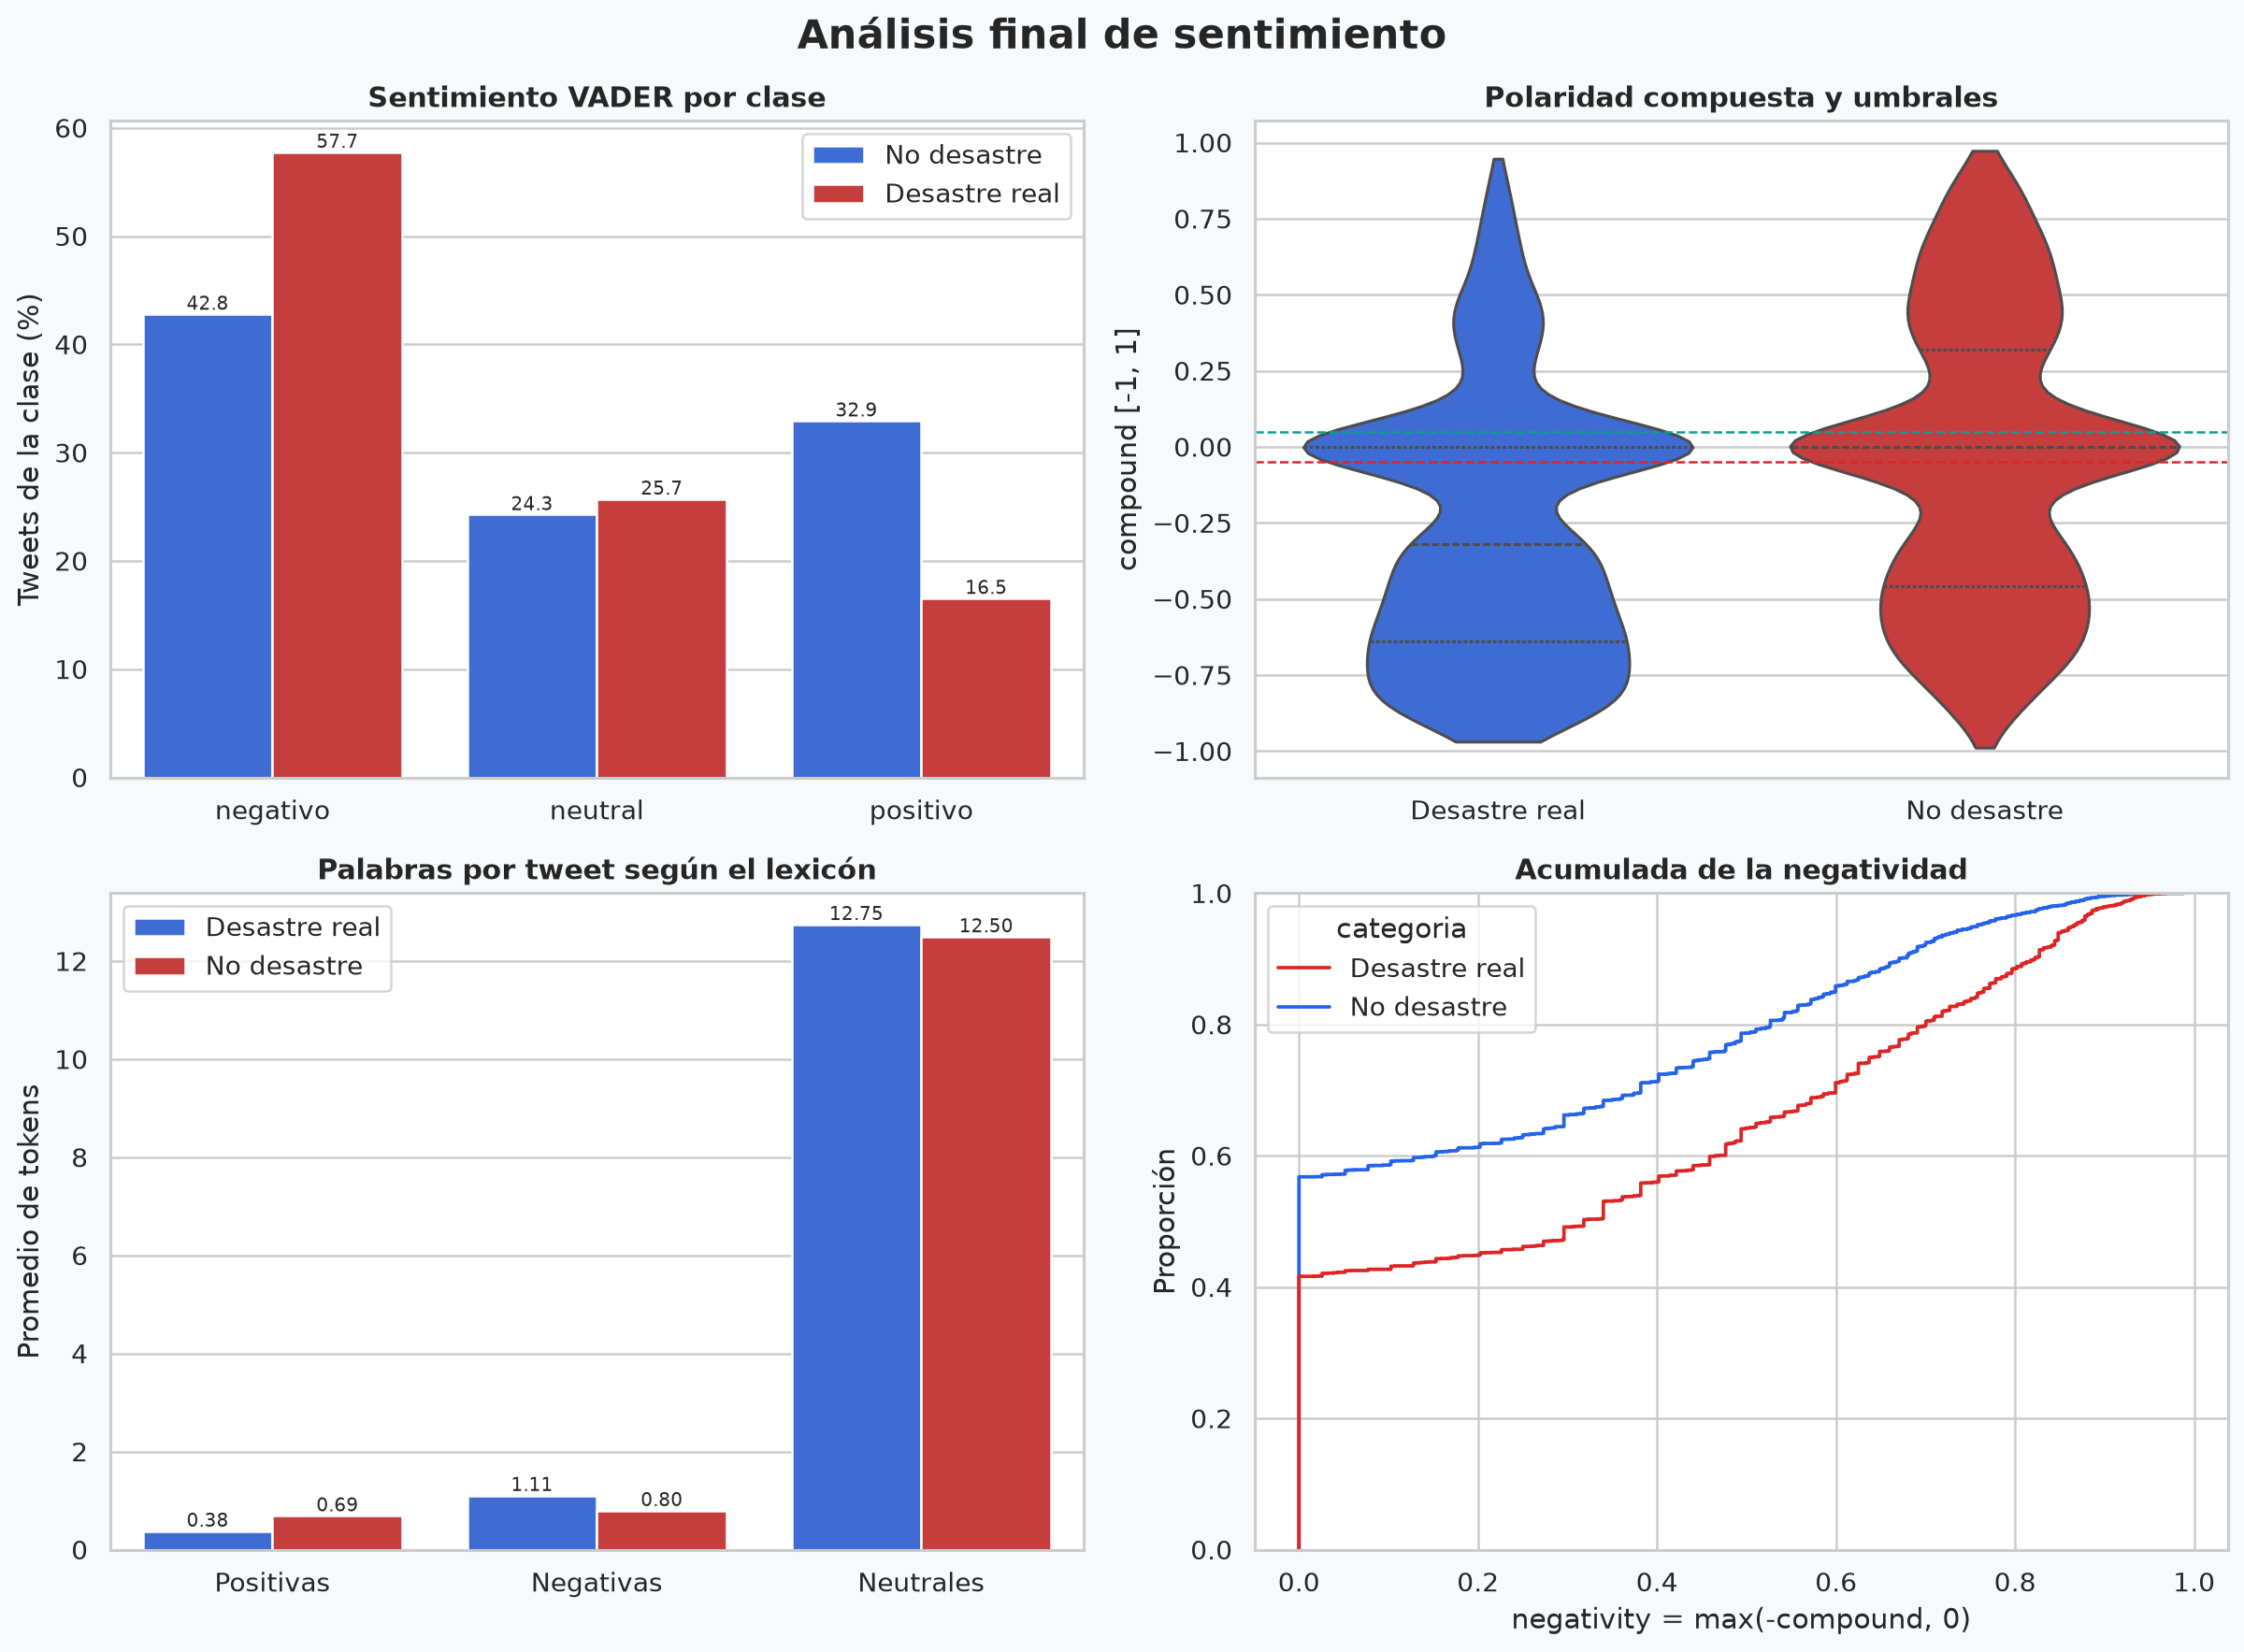
\includegraphics[width=0.98\textwidth]{../outputs/figures/sentimiento_final.png}
\caption{Distribución, intensidad y negatividad del sentimiento por clase.}
\label{fig:sentimiento}
\end{figure}

El sentimiento no es sinónimo de desastre. Un reporte factual puede ser neutral y una publicación personal puede expresar fuerte negatividad sin describir una emergencia real. Esta separación conceptual motiva el experimento de aporte incremental de la Sección \ref{sec:negatividad}.

\subsection{Tweets extremos}

Se ordenó el corpus por \texttt{compound} y se seleccionaron los diez valores más altos y los diez más bajos. Siete de los diez extremos negativos corresponden a desastres; nueve de los diez extremos positivos son de la clase sin desastre. Los negativos contienen muerte, lesión, amenaza y destrucción. Los positivos concentran agradecimiento, apoyo, humor y mensajes promocionales. Las tablas completas preservan identificador, texto, clase y puntajes para que la interpretación sea verificable.

\begin{figure}[H]
\centering
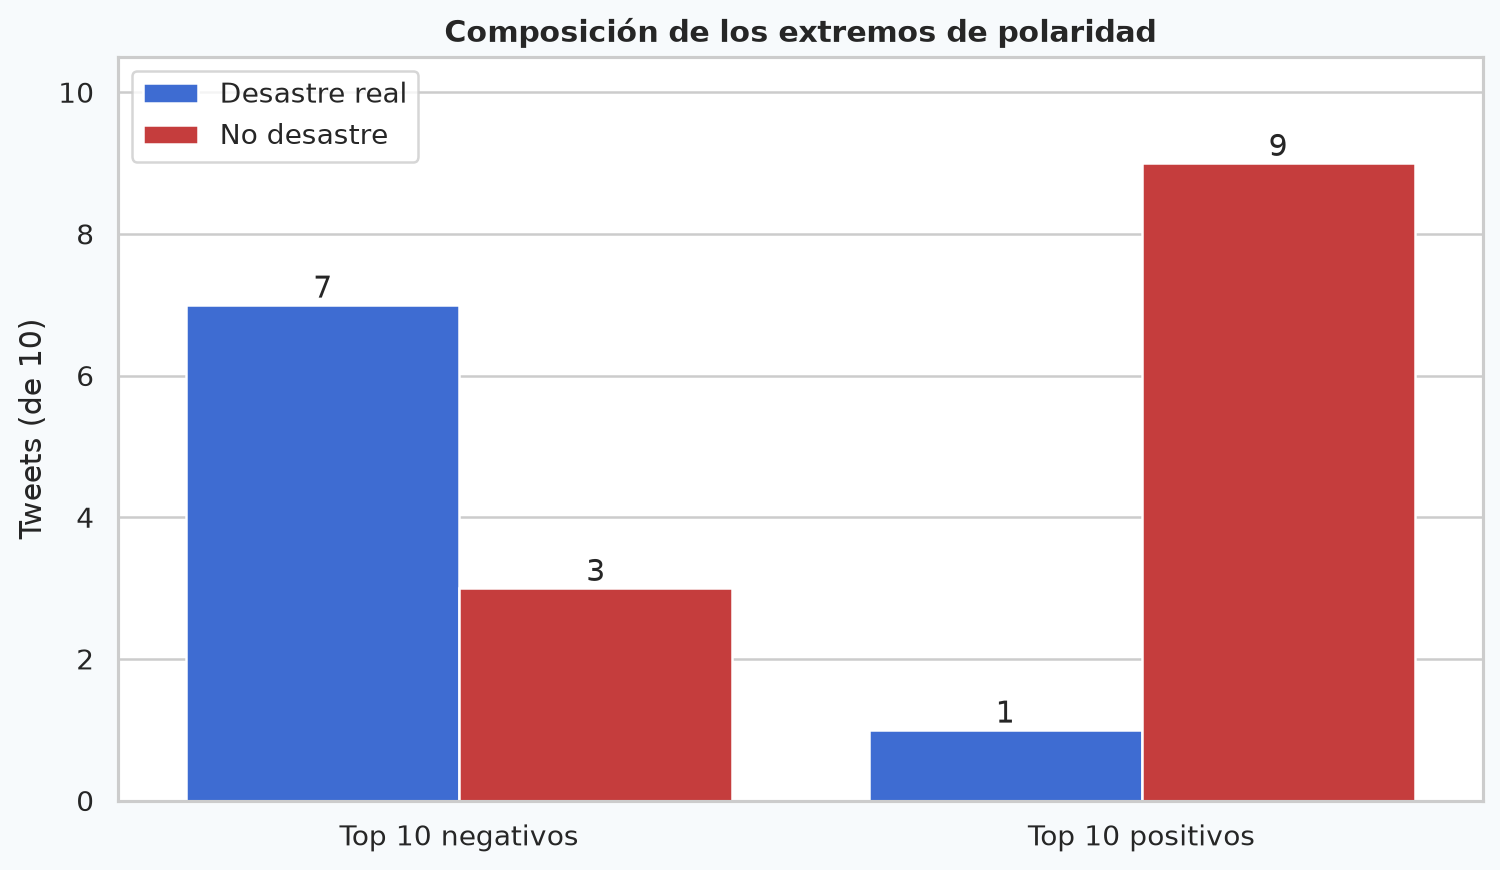
\includegraphics[width=0.72\textwidth]{../outputs/figures/top10_composicion.png}
\caption{Composición por clase de los diez tweets más positivos y negativos.}
\label{fig:top10}
\end{figure}

\section{Contraste de negatividad}

Se definió una variable no negativa:
\[
  negativity_i = \max(-compound_i,0).
\]

El 50.28\% de las observaciones tiene valor cero. Dada la masa en cero y la asimetría, se utilizó Mann--Whitney bilateral en vez de una prueba paramétrica. La diferencia de medias se complementó con un intervalo bootstrap del 95\% y delta de Cliff como tamaño de efecto.

\begin{table}[H]
\centering
\caption{Comparación de negatividad entre clases.}
\label{tab:contraste}
\begin{tabular}{lr}
\toprule
Indicador & Resultado\\
\midrule
Media, desastre real & 0.3366\\
Media, no desastre & 0.2126\\
Diferencia de medias & 0.1240\\
IC bootstrap 95\% & [0.1099, 0.1382]\\
Valor \(p\), Mann--Whitney & \(<0.001\)\\
Delta de Cliff & 0.2069 (pequeño)\\
\bottomrule
\end{tabular}
\end{table}

El resultado respalda que los tweets de desastre son más negativos en distribución, pero la magnitud pequeña anticipa que la variable por sí sola no separará perfectamente las clases.

\begin{figure}[H]
\centering
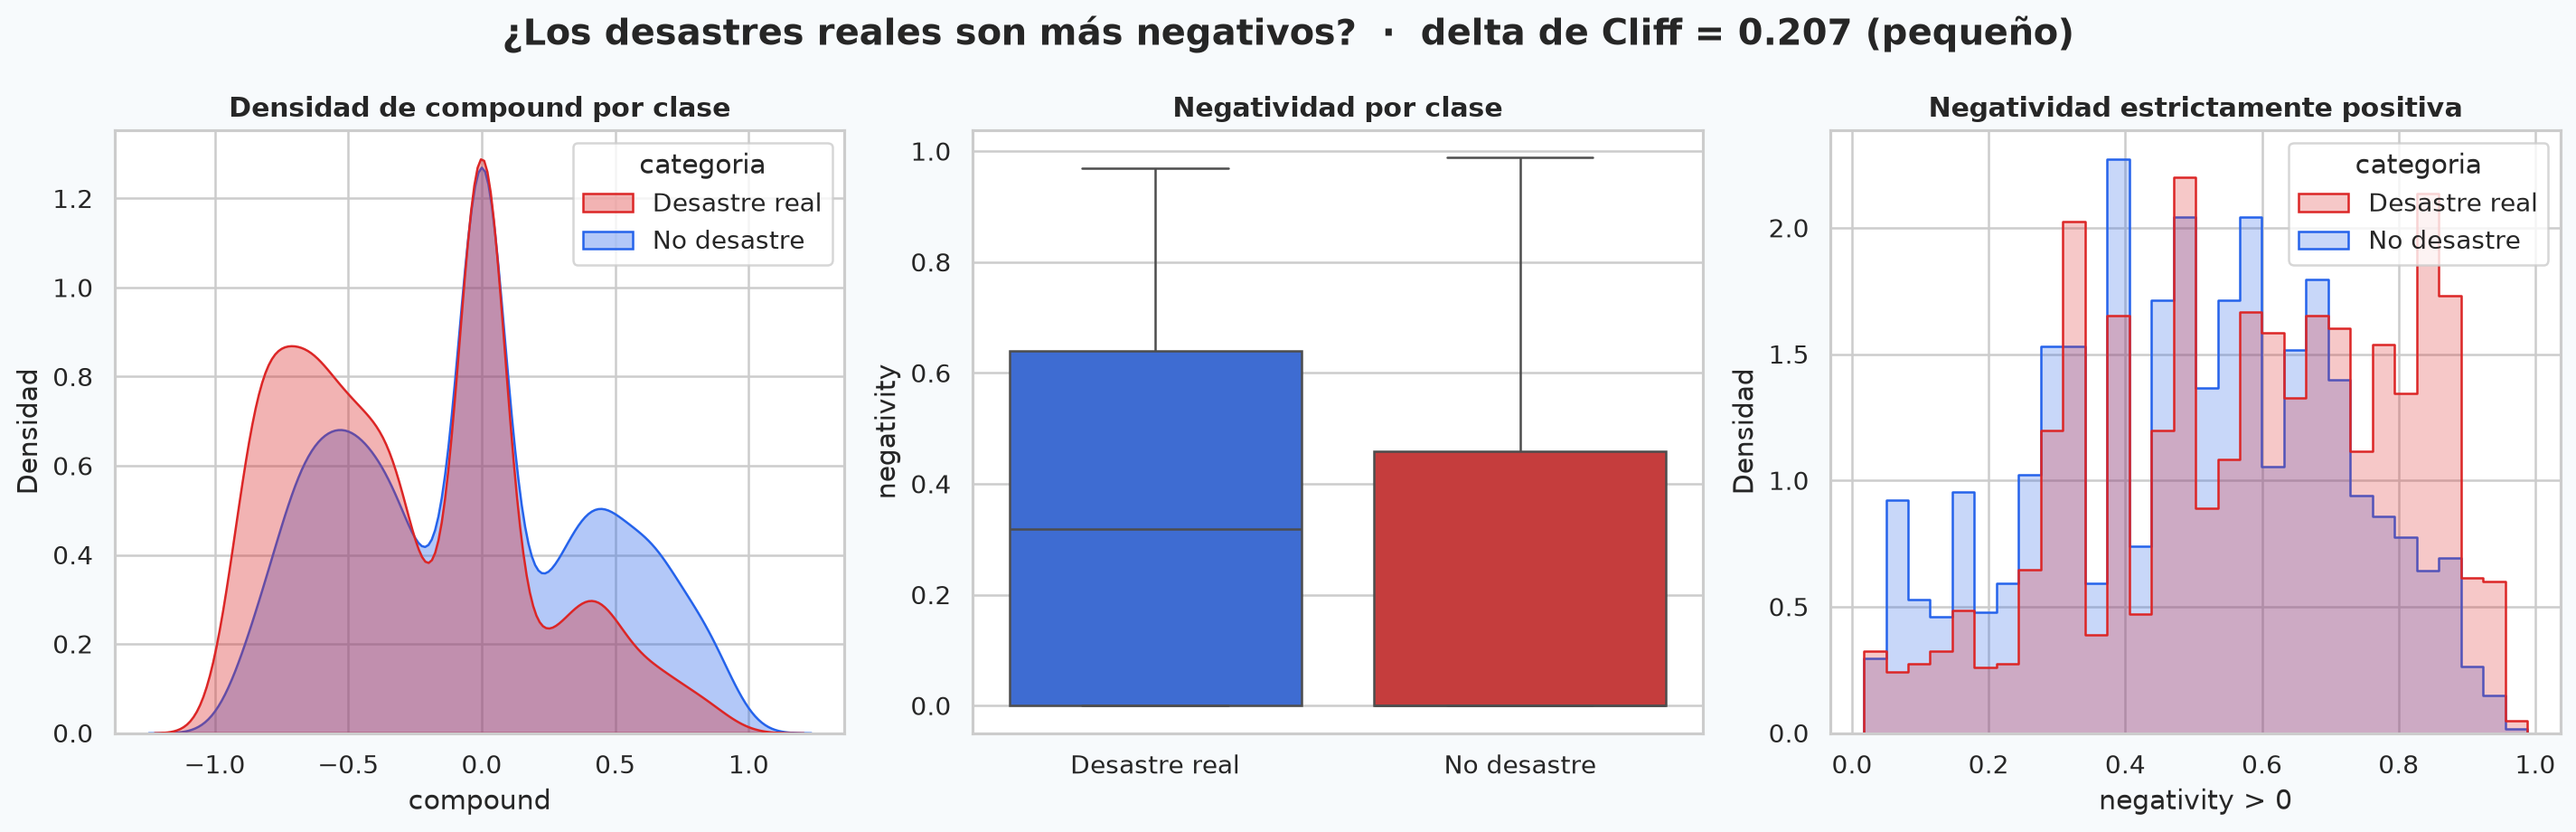
\includegraphics[width=0.98\textwidth]{../outputs/figures/contraste_negatividad.png}
\caption{Contraste descriptivo e inferencial de la negatividad.}
\label{fig:contraste}
\end{figure}

\section{Reentrenamiento con negatividad}\label{sec:negatividad}

Se compararon dos pipelines bajo la misma división: A, regresión logística con TF--IDF; y B, la misma representación más \texttt{negativity}. No se cambiaron hiperparámetros ni observaciones.

\begin{table}[H]
\centering
\caption{Efecto de incorporar la variable de negatividad.}
\label{tab:ab}
\small
\begin{tabular}{lrrr}
\toprule
Métrica & A: sin negatividad & B: con negatividad & Diferencia B--A\\
\midrule
Exactitud & 0.8129 & 0.7978 & -0.0151\\
Precisión & 0.7852 & 0.7662 & -0.0190\\
Recall & 0.7768 & 0.7615 & -0.0153\\
F1 & 0.7809 & 0.7638 & -0.0171\\
F1 macro & 0.8088 & 0.7935 & -0.0153\\
ROC--AUC & 0.8666 & 0.8670 & +0.0004\\
Falsos positivos & 139 & 152 & +13\\
Falsos negativos & 146 & 156 & +10\\
\bottomrule
\end{tabular}
\end{table}

La mejora mínima de ROC--AUC no compensa el deterioro del resto de métricas. La negatividad probablemente es redundante con términos que TF--IDF ya representa. En consecuencia, el modelo final es A y se registra explícitamente que no usa la variable adicional.

\begin{figure}[H]
\centering
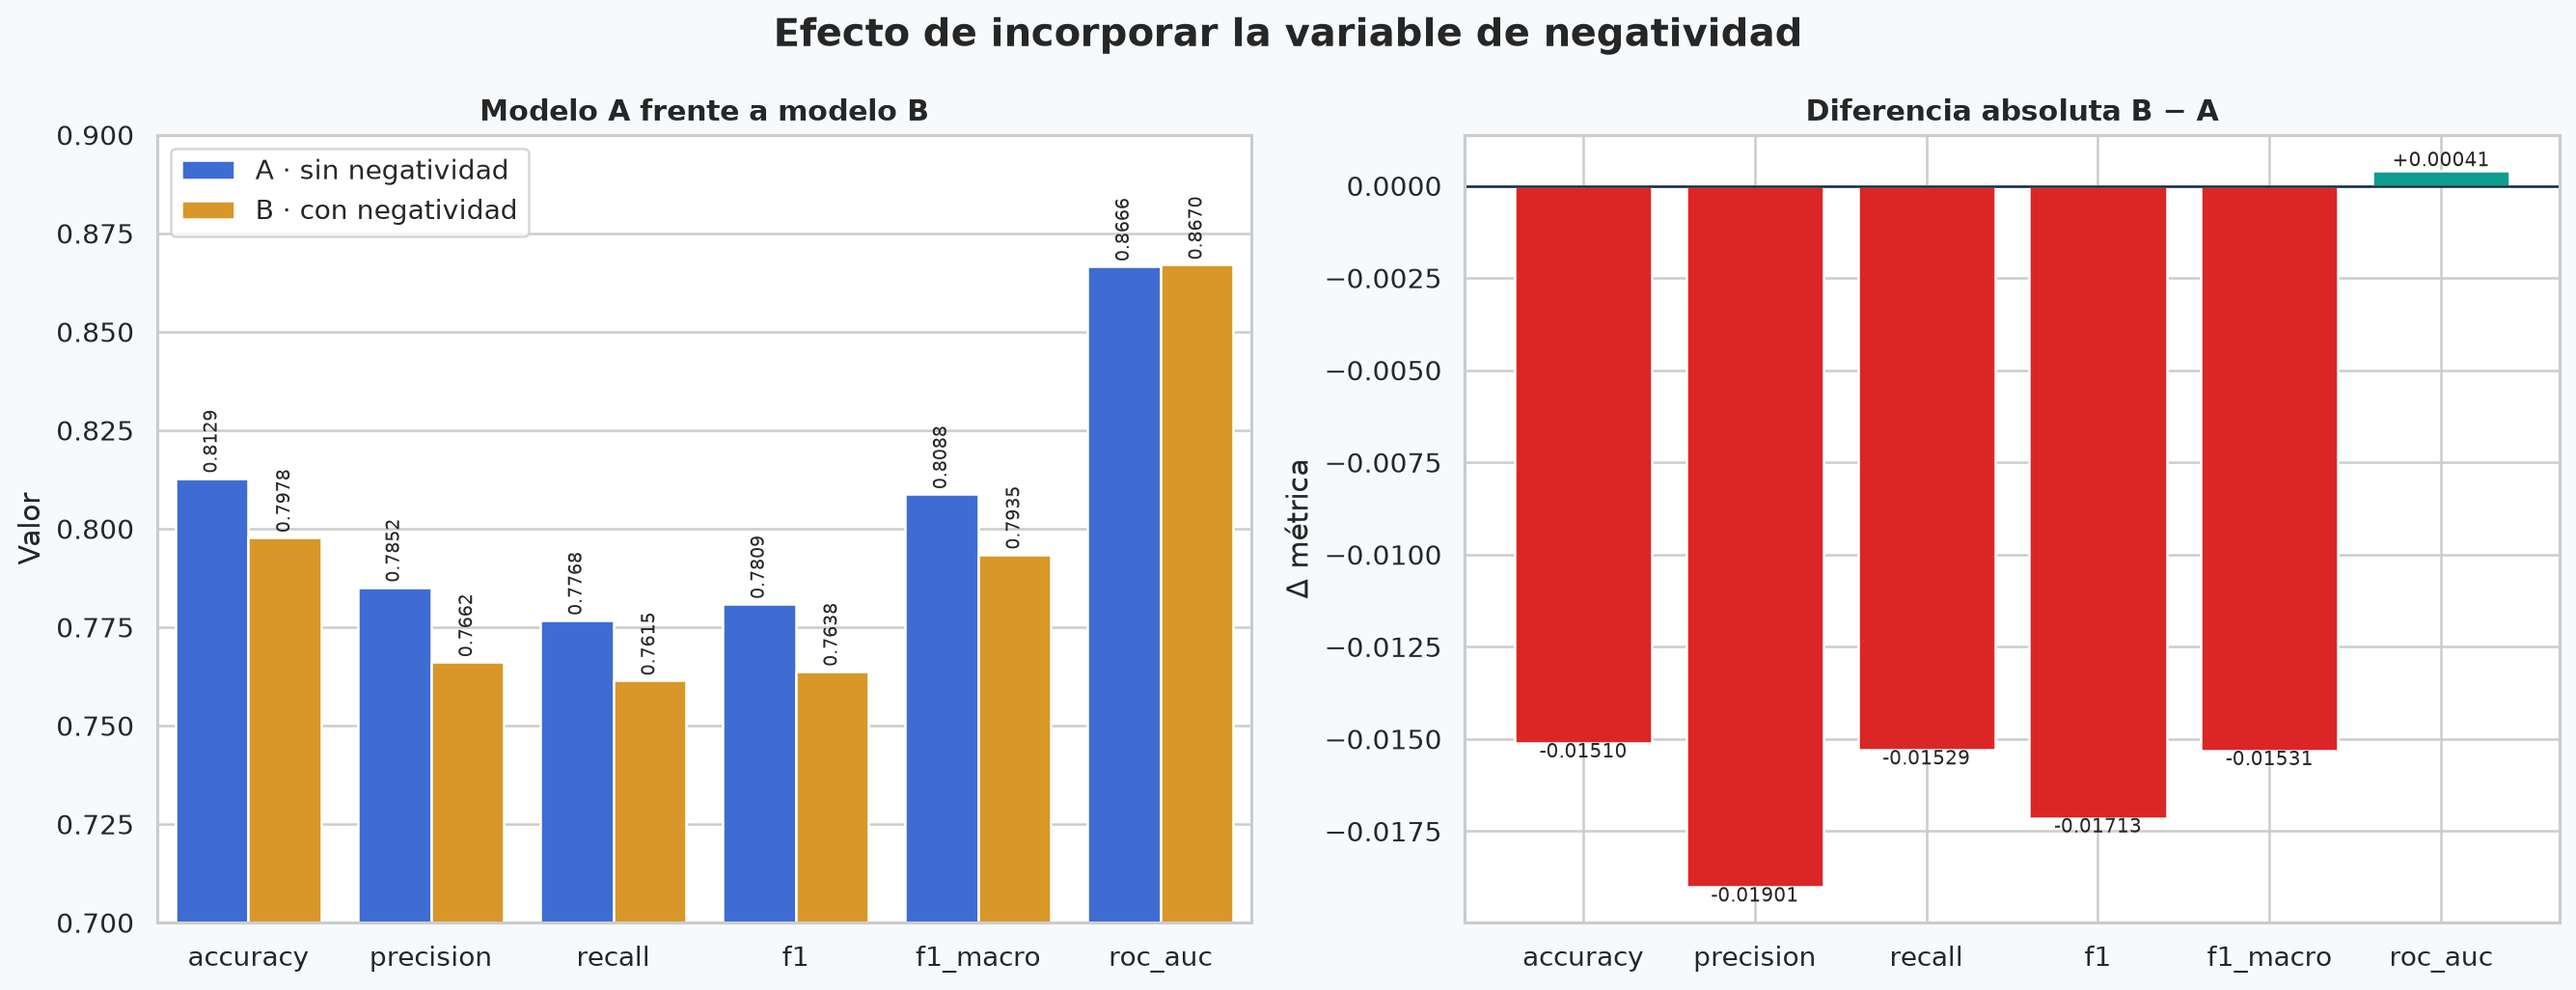
\includegraphics[width=0.97\textwidth]{../outputs/figures/comparacion_negatividad.png}
\caption{Comparación controlada de desempeño con y sin negatividad.}
\label{fig:ab}
\end{figure}

\section{Análisis de errores y discusión}

El modelo final produce 139 falsos positivos y 146 falsos negativos. Los falsos positivos suelen contener vocabulario alarmante en contextos figurados, humorísticos o promocionales. Los falsos negativos incluyen mensajes breves, ubicaciones implícitas y reportes factuales cuyo tono no es abiertamente negativo.

\begin{figure}[H]
\centering
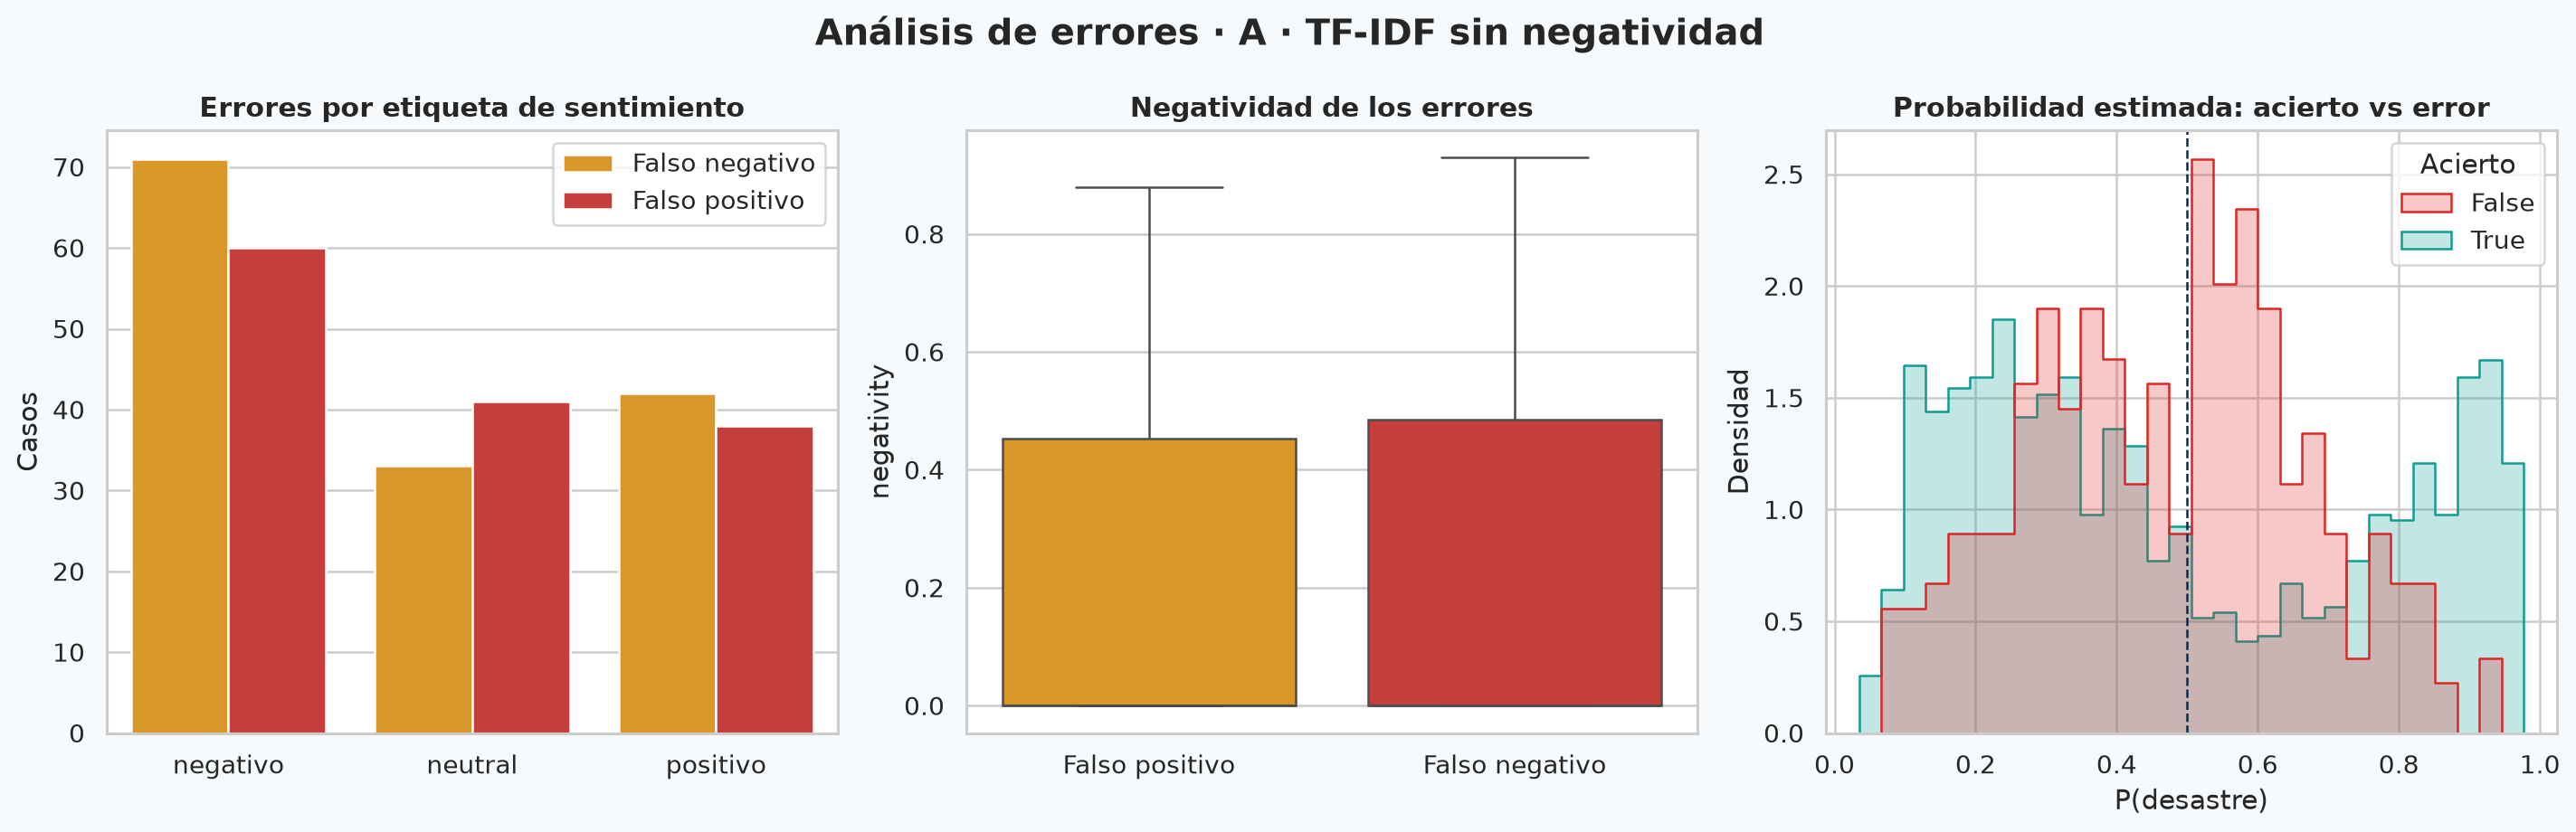
\includegraphics[width=0.98\textwidth]{../outputs/figures/analisis_errores.png}
\caption{Distribución de errores según sentimiento, negatividad y probabilidad estimada.}
\label{fig:errores}
\end{figure}

Los errores cercanos a probabilidad 0.5 representan ambigüedad esperable. Los errores de alta confianza son más relevantes: exhiben ironía, metáforas, titulares sin contexto y referencias que exigen conocimiento externo. Un modelo lineal con bolsa de palabras no comprende de forma explícita temporalidad, causalidad o sarcasmo.

\subsection{Limitaciones}

\begin{itemize}
  \item El corpus fue construido para una competencia y puede no representar todas las emergencias, regiones o variedades lingüísticas.
  \item VADER fue diseñado para inglés y redes sociales; sus reglas no constituyen una medición clínica ni causal de emociones.
  \item Se utiliza una sola partición estratificada. La semilla fija permite reproducción, pero validación cruzada o un conjunto externo darían una estimación más estable.
  \item La lista estándar de palabras vacías elimina algunos términos de contenido; el fenómeno se auditó, pero futuros trabajos podrían diseñar una lista específica del dominio.
  \item La significancia estadística no implica utilidad predictiva, como demuestra el experimento con negatividad.
\end{itemize}

\section{Conclusiones}

\begin{enumerate}
  \item La representación TF--IDF de unigramas y bigramas captura suficiente contexto para superar ampliamente el baseline.
  \item La regresión logística alcanza el mejor F1 de la comparación y ofrece un modelo transparente, ligero y reproducible.
  \item Los tweets de desastres reales son más negativos en promedio; la evidencia inferencial es fuerte, aunque el tamaño de efecto es pequeño.
  \item La variable de negatividad no mejora el modelo: reduce exactitud, precisión, recall y F1. Por ello se excluye del clasificador definitivo.
  \item El análisis de errores muestra que la principal frontera pendiente es semántica: ironía, lenguaje figurado y contexto ausente requieren representaciones más ricas.
  \item El repositorio entrega código modular, notebook ejecutado, tablas, figuras, pruebas, modelo persistido, metadatos e informe, lo que permite verificar cada resultado.
\end{enumerate}

\section{Reproducibilidad y trazabilidad}

El entorno se instala desde \texttt{pyproject.toml}, \texttt{uv.lock} o \texttt{requirements.txt}. El flujo se divide en cuatro comandos verificables:
\begin{itemize}
  \item etapa base: \texttt{scripts/run\_advance.py};
  \item análisis y modelo final: \texttt{scripts/run\_final.py};
  \item notebook narrativo: \texttt{scripts/build\_notebook.py};
  \item inferencia individual: \texttt{scripts/predict\_tweet.py}.
\end{itemize}
La suite automatizada comprueba fórmulas, limpieza, partición, contrato de resultados, persistencia del modelo y metadatos.

La tabla \texttt{outputs/tables/evidencia\_rubrica.csv} enlaza cada criterio con archivos concretos y comprueba su existencia. El historial del código y los entregables está disponible en \repo.

\begin{thebibliography}{9}
\bibitem{vader}
Hutto, C. J. y Gilbert, E. (2014). \emph{VADER: A Parsimonious Rule-based Model for Sentiment Analysis of Social Media Text}. Proceedings of the International AAAI Conference on Web and Social Media.

\bibitem{sklearn}
Pedregosa, F. et al. (2011). \emph{Scikit-learn: Machine Learning in Python}. Journal of Machine Learning Research, 12, 2825--2830.

\bibitem{tfidf}
Salton, G. y Buckley, C. (1988). \emph{Term-weighting approaches in automatic text retrieval}. Information Processing \& Management, 24(5), 513--523.

\bibitem{kaggle}
Kaggle. \emph{Natural Language Processing with Disaster Tweets}. \url{https://www.kaggle.com/competitions/nlp-getting-started}. Consultado en 2026.

\bibitem{scikittext}
Scikit-learn Developers. \emph{Working With Text Data}. \url{https://scikit-learn.org/stable/tutorial/text_analytics/working_with_text_data.html}. Consultado en 2026.
\end{thebibliography}

\appendix
\section{Correspondencia con la rúbrica}

\begin{longtable}{p{0.39\textwidth}p{0.52\textwidth}}
\toprule
\textbf{Criterio} & \textbf{Evidencia principal}\\
\midrule
EDA & Figura \ref{fig:eda}, \texttt{eda\_por\_clase.csv}\\
Limpieza y preprocesamiento & \texttt{auditoria\_limpieza.csv}, ejemplos y auditoría de stopwords\\
N-gramas, frecuencias y probabilidades & Figura \ref{fig:ngrams} y tablas por clase\\
Modelos clasificadores & Tabla \ref{tab:modelos}, Figuras \ref{fig:confusion} y \ref{fig:ab}\\
Función de clasificación & \texttt{classify\_raw\_tweet}, \texttt{predict\_tweet.py}, modelo persistido\\
Sentimiento & Figura \ref{fig:sentimiento}, umbrales y tablas de distribución\\
Variable de negatividad & Tabla \ref{tab:ab} y contraste controlado A/B\\
Resultados y discusión & Figuras \ref{fig:contraste} y \ref{fig:errores}, conclusiones y limitaciones\\
\bottomrule
\end{longtable}

\end{document}
